% Created by tikzDevice version 0.12 on 2019-05-08 13:29:01
% !TEX encoding = UTF-8 Unicode
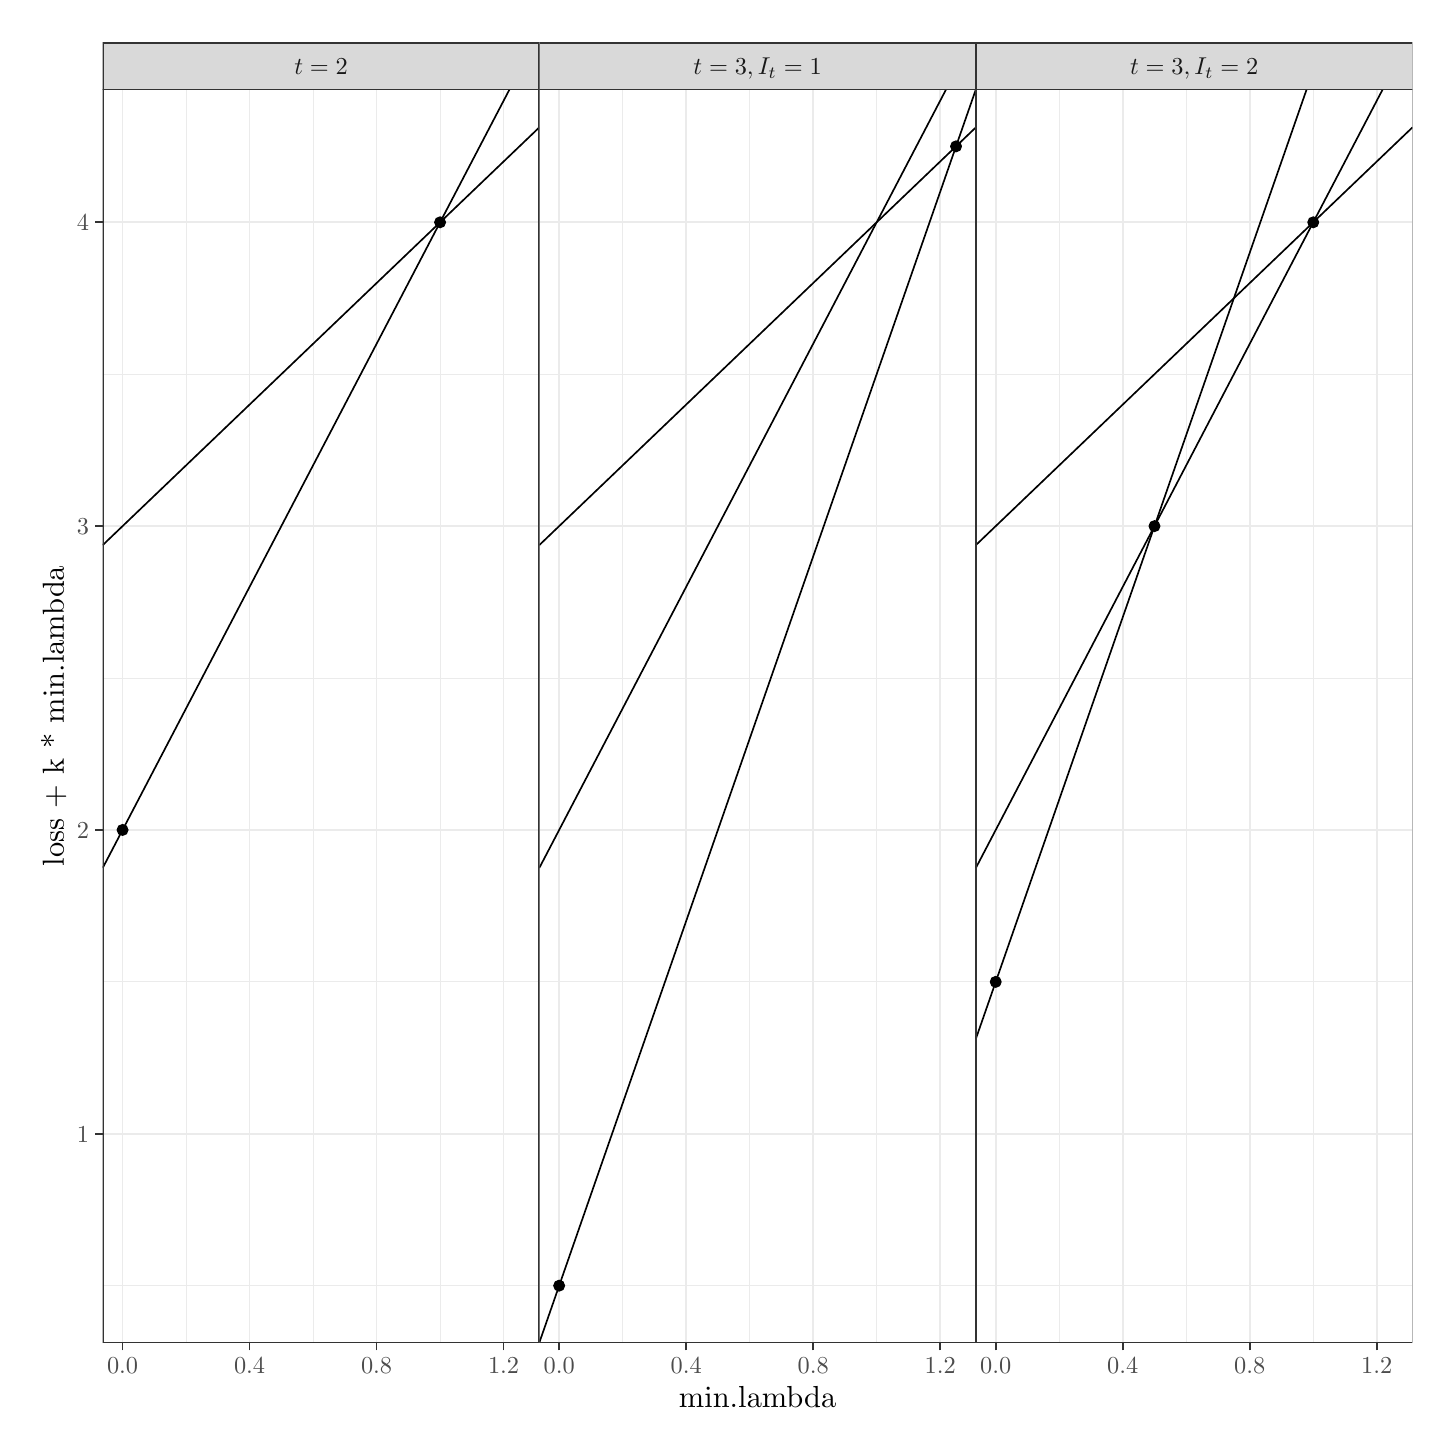
\begin{tikzpicture}[x=1pt,y=1pt]
\definecolor{fillColor}{RGB}{255,255,255}
\path[use as bounding box,fill=fillColor,fill opacity=0.00] (0,0) rectangle (505.89,505.89);
\begin{scope}
\path[clip] (  0.00,  0.00) rectangle (505.89,505.89);
\definecolor{drawColor}{RGB}{255,255,255}
\definecolor{fillColor}{RGB}{255,255,255}

\path[draw=drawColor,line width= 0.6pt,line join=round,line cap=round,fill=fillColor] (  0.00,  0.00) rectangle (505.89,505.89);
\end{scope}
\begin{scope}
\path[clip] ( 27.12, 30.72) rectangle (184.88,483.59);
\definecolor{fillColor}{RGB}{255,255,255}

\path[fill=fillColor] ( 27.12, 30.72) rectangle (184.88,483.59);
\definecolor{drawColor}{gray}{0.92}

\path[draw=drawColor,line width= 0.3pt,line join=round] ( 27.12, 51.31) --
	(184.88, 51.31);

\path[draw=drawColor,line width= 0.3pt,line join=round] ( 27.12,161.09) --
	(184.88,161.09);

\path[draw=drawColor,line width= 0.3pt,line join=round] ( 27.12,270.88) --
	(184.88,270.88);

\path[draw=drawColor,line width= 0.3pt,line join=round] ( 27.12,380.66) --
	(184.88,380.66);

\path[draw=drawColor,line width= 0.3pt,line join=round] ( 57.24, 30.72) --
	( 57.24,483.59);

\path[draw=drawColor,line width= 0.3pt,line join=round] (103.13, 30.72) --
	(103.13,483.59);

\path[draw=drawColor,line width= 0.3pt,line join=round] (149.02, 30.72) --
	(149.02,483.59);

\path[draw=drawColor,line width= 0.6pt,line join=round] ( 27.12,106.20) --
	(184.88,106.20);

\path[draw=drawColor,line width= 0.6pt,line join=round] ( 27.12,215.99) --
	(184.88,215.99);

\path[draw=drawColor,line width= 0.6pt,line join=round] ( 27.12,325.77) --
	(184.88,325.77);

\path[draw=drawColor,line width= 0.6pt,line join=round] ( 27.12,435.55) --
	(184.88,435.55);

\path[draw=drawColor,line width= 0.6pt,line join=round] ( 34.29, 30.72) --
	( 34.29,483.59);

\path[draw=drawColor,line width= 0.6pt,line join=round] ( 80.18, 30.72) --
	( 80.18,483.59);

\path[draw=drawColor,line width= 0.6pt,line join=round] (126.08, 30.72) --
	(126.08,483.59);

\path[draw=drawColor,line width= 0.6pt,line join=round] (171.97, 30.72) --
	(171.97,483.59);
\definecolor{drawColor}{RGB}{0,0,0}
\definecolor{fillColor}{RGB}{0,0,0}

\path[draw=drawColor,line width= 0.4pt,line join=round,line cap=round,fill=fillColor] ( 34.29,215.99) circle (  1.96);

\path[draw=drawColor,line width= 0.4pt,line join=round,line cap=round,fill=fillColor] (149.02,435.55) circle (  1.96);

\path[draw=drawColor,line width= 0.6pt,line join=round] ( 27.12,318.91) -- (184.88,469.86);

\path[draw=drawColor,line width= 0.6pt,line join=round] ( 27.12,202.26) -- (184.88,504.17);
\definecolor{drawColor}{gray}{0.20}

\path[draw=drawColor,line width= 0.6pt,line join=round,line cap=round] ( 27.12, 30.72) rectangle (184.88,483.59);
\end{scope}
\begin{scope}
\path[clip] (184.88, 30.72) rectangle (342.63,483.59);
\definecolor{fillColor}{RGB}{255,255,255}

\path[fill=fillColor] (184.88, 30.72) rectangle (342.63,483.59);
\definecolor{drawColor}{gray}{0.92}

\path[draw=drawColor,line width= 0.3pt,line join=round] (184.88, 51.31) --
	(342.63, 51.31);

\path[draw=drawColor,line width= 0.3pt,line join=round] (184.88,161.09) --
	(342.63,161.09);

\path[draw=drawColor,line width= 0.3pt,line join=round] (184.88,270.88) --
	(342.63,270.88);

\path[draw=drawColor,line width= 0.3pt,line join=round] (184.88,380.66) --
	(342.63,380.66);

\path[draw=drawColor,line width= 0.3pt,line join=round] (214.99, 30.72) --
	(214.99,483.59);

\path[draw=drawColor,line width= 0.3pt,line join=round] (260.89, 30.72) --
	(260.89,483.59);

\path[draw=drawColor,line width= 0.3pt,line join=round] (306.78, 30.72) --
	(306.78,483.59);

\path[draw=drawColor,line width= 0.6pt,line join=round] (184.88,106.20) --
	(342.63,106.20);

\path[draw=drawColor,line width= 0.6pt,line join=round] (184.88,215.99) --
	(342.63,215.99);

\path[draw=drawColor,line width= 0.6pt,line join=round] (184.88,325.77) --
	(342.63,325.77);

\path[draw=drawColor,line width= 0.6pt,line join=round] (184.88,435.55) --
	(342.63,435.55);

\path[draw=drawColor,line width= 0.6pt,line join=round] (192.05, 30.72) --
	(192.05,483.59);

\path[draw=drawColor,line width= 0.6pt,line join=round] (237.94, 30.72) --
	(237.94,483.59);

\path[draw=drawColor,line width= 0.6pt,line join=round] (283.83, 30.72) --
	(283.83,483.59);

\path[draw=drawColor,line width= 0.6pt,line join=round] (329.73, 30.72) --
	(329.73,483.59);
\definecolor{drawColor}{RGB}{0,0,0}
\definecolor{fillColor}{RGB}{0,0,0}

\path[draw=drawColor,line width= 0.4pt,line join=round,line cap=round,fill=fillColor] (192.05, 51.31) circle (  1.96);

\path[draw=drawColor,line width= 0.4pt,line join=round,line cap=round,fill=fillColor] (335.46,463.00) circle (  1.96);

\path[draw=drawColor,line width= 0.6pt,line join=round] (184.88,318.91) -- (342.63,469.86);

\path[draw=drawColor,line width= 0.6pt,line join=round] (184.88,202.26) -- (342.63,504.17);

\path[draw=drawColor,line width= 0.6pt,line join=round] (184.88, 30.72) -- (342.63,483.59);
\definecolor{drawColor}{gray}{0.20}

\path[draw=drawColor,line width= 0.6pt,line join=round,line cap=round] (184.88, 30.72) rectangle (342.63,483.59);
\end{scope}
\begin{scope}
\path[clip] (342.63, 30.72) rectangle (500.39,483.59);
\definecolor{fillColor}{RGB}{255,255,255}

\path[fill=fillColor] (342.63, 30.72) rectangle (500.39,483.59);
\definecolor{drawColor}{gray}{0.92}

\path[draw=drawColor,line width= 0.3pt,line join=round] (342.63, 51.31) --
	(500.39, 51.31);

\path[draw=drawColor,line width= 0.3pt,line join=round] (342.63,161.09) --
	(500.39,161.09);

\path[draw=drawColor,line width= 0.3pt,line join=round] (342.63,270.88) --
	(500.39,270.88);

\path[draw=drawColor,line width= 0.3pt,line join=round] (342.63,380.66) --
	(500.39,380.66);

\path[draw=drawColor,line width= 0.3pt,line join=round] (372.75, 30.72) --
	(372.75,483.59);

\path[draw=drawColor,line width= 0.3pt,line join=round] (418.64, 30.72) --
	(418.64,483.59);

\path[draw=drawColor,line width= 0.3pt,line join=round] (464.54, 30.72) --
	(464.54,483.59);

\path[draw=drawColor,line width= 0.6pt,line join=round] (342.63,106.20) --
	(500.39,106.20);

\path[draw=drawColor,line width= 0.6pt,line join=round] (342.63,215.99) --
	(500.39,215.99);

\path[draw=drawColor,line width= 0.6pt,line join=round] (342.63,325.77) --
	(500.39,325.77);

\path[draw=drawColor,line width= 0.6pt,line join=round] (342.63,435.55) --
	(500.39,435.55);

\path[draw=drawColor,line width= 0.6pt,line join=round] (349.80, 30.72) --
	(349.80,483.59);

\path[draw=drawColor,line width= 0.6pt,line join=round] (395.70, 30.72) --
	(395.70,483.59);

\path[draw=drawColor,line width= 0.6pt,line join=round] (441.59, 30.72) --
	(441.59,483.59);

\path[draw=drawColor,line width= 0.6pt,line join=round] (487.48, 30.72) --
	(487.48,483.59);
\definecolor{drawColor}{RGB}{0,0,0}
\definecolor{fillColor}{RGB}{0,0,0}

\path[draw=drawColor,line width= 0.4pt,line join=round,line cap=round,fill=fillColor] (349.80,161.09) circle (  1.96);

\path[draw=drawColor,line width= 0.4pt,line join=round,line cap=round,fill=fillColor] (407.17,325.77) circle (  1.96);

\path[draw=drawColor,line width= 0.4pt,line join=round,line cap=round,fill=fillColor] (464.54,435.55) circle (  1.96);

\path[draw=drawColor,line width= 0.6pt,line join=round] (342.63,318.91) -- (500.39,469.86);

\path[draw=drawColor,line width= 0.6pt,line join=round] (342.63,202.26) -- (500.39,504.17);

\path[draw=drawColor,line width= 0.6pt,line join=round] (342.63,140.51) -- (469.92,505.89);
\definecolor{drawColor}{gray}{0.20}

\path[draw=drawColor,line width= 0.6pt,line join=round,line cap=round] (342.63, 30.72) rectangle (500.39,483.59);
\end{scope}
\begin{scope}
\path[clip] ( 27.12,483.59) rectangle (184.88,500.39);
\definecolor{drawColor}{gray}{0.20}
\definecolor{fillColor}{gray}{0.85}

\path[draw=drawColor,line width= 0.6pt,line join=round,line cap=round,fill=fillColor] ( 27.12,483.59) rectangle (184.88,500.39);
\definecolor{drawColor}{gray}{0.10}

\node[text=drawColor,anchor=base,inner sep=0pt, outer sep=0pt, scale=  0.88] at (106.00,488.96) {$t=2$};
\end{scope}
\begin{scope}
\path[clip] (184.88,483.59) rectangle (342.63,500.39);
\definecolor{drawColor}{gray}{0.20}
\definecolor{fillColor}{gray}{0.85}

\path[draw=drawColor,line width= 0.6pt,line join=round,line cap=round,fill=fillColor] (184.88,483.59) rectangle (342.63,500.39);
\definecolor{drawColor}{gray}{0.10}

\node[text=drawColor,anchor=base,inner sep=0pt, outer sep=0pt, scale=  0.88] at (263.75,488.96) {$t=3, I_t=1$};
\end{scope}
\begin{scope}
\path[clip] (342.63,483.59) rectangle (500.39,500.39);
\definecolor{drawColor}{gray}{0.20}
\definecolor{fillColor}{gray}{0.85}

\path[draw=drawColor,line width= 0.6pt,line join=round,line cap=round,fill=fillColor] (342.63,483.59) rectangle (500.39,500.39);
\definecolor{drawColor}{gray}{0.10}

\node[text=drawColor,anchor=base,inner sep=0pt, outer sep=0pt, scale=  0.88] at (421.51,488.96) {$t=3, I_t=2$};
\end{scope}
\begin{scope}
\path[clip] (  0.00,  0.00) rectangle (505.89,505.89);
\definecolor{drawColor}{gray}{0.20}

\path[draw=drawColor,line width= 0.6pt,line join=round] ( 34.29, 27.97) --
	( 34.29, 30.72);

\path[draw=drawColor,line width= 0.6pt,line join=round] ( 80.18, 27.97) --
	( 80.18, 30.72);

\path[draw=drawColor,line width= 0.6pt,line join=round] (126.08, 27.97) --
	(126.08, 30.72);

\path[draw=drawColor,line width= 0.6pt,line join=round] (171.97, 27.97) --
	(171.97, 30.72);
\end{scope}
\begin{scope}
\path[clip] (  0.00,  0.00) rectangle (505.89,505.89);
\definecolor{drawColor}{gray}{0.30}

\node[text=drawColor,anchor=base,inner sep=0pt, outer sep=0pt, scale=  0.88] at ( 34.29, 19.71) {0.0};

\node[text=drawColor,anchor=base,inner sep=0pt, outer sep=0pt, scale=  0.88] at ( 80.18, 19.71) {0.4};

\node[text=drawColor,anchor=base,inner sep=0pt, outer sep=0pt, scale=  0.88] at (126.08, 19.71) {0.8};

\node[text=drawColor,anchor=base,inner sep=0pt, outer sep=0pt, scale=  0.88] at (171.97, 19.71) {1.2};
\end{scope}
\begin{scope}
\path[clip] (  0.00,  0.00) rectangle (505.89,505.89);
\definecolor{drawColor}{gray}{0.20}

\path[draw=drawColor,line width= 0.6pt,line join=round] (192.05, 27.97) --
	(192.05, 30.72);

\path[draw=drawColor,line width= 0.6pt,line join=round] (237.94, 27.97) --
	(237.94, 30.72);

\path[draw=drawColor,line width= 0.6pt,line join=round] (283.83, 27.97) --
	(283.83, 30.72);

\path[draw=drawColor,line width= 0.6pt,line join=round] (329.73, 27.97) --
	(329.73, 30.72);
\end{scope}
\begin{scope}
\path[clip] (  0.00,  0.00) rectangle (505.89,505.89);
\definecolor{drawColor}{gray}{0.30}

\node[text=drawColor,anchor=base,inner sep=0pt, outer sep=0pt, scale=  0.88] at (192.05, 19.71) {0.0};

\node[text=drawColor,anchor=base,inner sep=0pt, outer sep=0pt, scale=  0.88] at (237.94, 19.71) {0.4};

\node[text=drawColor,anchor=base,inner sep=0pt, outer sep=0pt, scale=  0.88] at (283.83, 19.71) {0.8};

\node[text=drawColor,anchor=base,inner sep=0pt, outer sep=0pt, scale=  0.88] at (329.73, 19.71) {1.2};
\end{scope}
\begin{scope}
\path[clip] (  0.00,  0.00) rectangle (505.89,505.89);
\definecolor{drawColor}{gray}{0.20}

\path[draw=drawColor,line width= 0.6pt,line join=round] (349.80, 27.97) --
	(349.80, 30.72);

\path[draw=drawColor,line width= 0.6pt,line join=round] (395.70, 27.97) --
	(395.70, 30.72);

\path[draw=drawColor,line width= 0.6pt,line join=round] (441.59, 27.97) --
	(441.59, 30.72);

\path[draw=drawColor,line width= 0.6pt,line join=round] (487.48, 27.97) --
	(487.48, 30.72);
\end{scope}
\begin{scope}
\path[clip] (  0.00,  0.00) rectangle (505.89,505.89);
\definecolor{drawColor}{gray}{0.30}

\node[text=drawColor,anchor=base,inner sep=0pt, outer sep=0pt, scale=  0.88] at (349.80, 19.71) {0.0};

\node[text=drawColor,anchor=base,inner sep=0pt, outer sep=0pt, scale=  0.88] at (395.70, 19.71) {0.4};

\node[text=drawColor,anchor=base,inner sep=0pt, outer sep=0pt, scale=  0.88] at (441.59, 19.71) {0.8};

\node[text=drawColor,anchor=base,inner sep=0pt, outer sep=0pt, scale=  0.88] at (487.48, 19.71) {1.2};
\end{scope}
\begin{scope}
\path[clip] (  0.00,  0.00) rectangle (505.89,505.89);
\definecolor{drawColor}{gray}{0.30}

\node[text=drawColor,anchor=base east,inner sep=0pt, outer sep=0pt, scale=  0.88] at ( 22.17,103.17) {1};

\node[text=drawColor,anchor=base east,inner sep=0pt, outer sep=0pt, scale=  0.88] at ( 22.17,212.96) {2};

\node[text=drawColor,anchor=base east,inner sep=0pt, outer sep=0pt, scale=  0.88] at ( 22.17,322.74) {3};

\node[text=drawColor,anchor=base east,inner sep=0pt, outer sep=0pt, scale=  0.88] at ( 22.17,432.52) {4};
\end{scope}
\begin{scope}
\path[clip] (  0.00,  0.00) rectangle (505.89,505.89);
\definecolor{drawColor}{gray}{0.20}

\path[draw=drawColor,line width= 0.6pt,line join=round] ( 24.37,106.20) --
	( 27.12,106.20);

\path[draw=drawColor,line width= 0.6pt,line join=round] ( 24.37,215.99) --
	( 27.12,215.99);

\path[draw=drawColor,line width= 0.6pt,line join=round] ( 24.37,325.77) --
	( 27.12,325.77);

\path[draw=drawColor,line width= 0.6pt,line join=round] ( 24.37,435.55) --
	( 27.12,435.55);
\end{scope}
\begin{scope}
\path[clip] (  0.00,  0.00) rectangle (505.89,505.89);
\definecolor{drawColor}{RGB}{0,0,0}

\node[text=drawColor,anchor=base,inner sep=0pt, outer sep=0pt, scale=  1.10] at (263.75,  7.44) {min.lambda};
\end{scope}
\begin{scope}
\path[clip] (  0.00,  0.00) rectangle (505.89,505.89);
\definecolor{drawColor}{RGB}{0,0,0}

\node[text=drawColor,rotate= 90.00,anchor=base,inner sep=0pt, outer sep=0pt, scale=  1.10] at ( 13.08,257.15) {loss + k * min.lambda};
\end{scope}
\end{tikzpicture}
